\documentclass{acm_proc_article-sp}
\usepackage{graphicx}
\usepackage{epsfig}
\usepackage{amsmath,amssymb}
\usepackage{cite}
\usepackage{url}
\usepackage{algorithm}
\usepackage{algorithmic}
\usepackage{listings}
% $Id$
\title{Dynamic Priority Search Tree Made Easy}
\author{$HeadURL: svn://192.168.69.130/usr/local/svnroot/lineda/pstme/pstme2.tex $,
        $Revision: 1786 $ }
\date{\today}

\newtheorem{theorem}{Theorem}

% workaround the old version of alogrithm package
\newcommand{\RETURN}{\STATE {\bf return} }

\begin{document}
\lstset{language=C++}
\maketitle

\begin{abstract}
We propose a data structure in our own version, the
Dynamic Priority Search Tree (PST). It is particularly for 2-D range
query in form of ($[x1:x2],[-\infty:y]$) and
($[x1:\infty],[-\infty:y]$). The Dynamic PST (DPST) allows dynamic
insertions and deletions while it maintains itself balanced. A
DPST takes O($\log n+m$) time for search. Insertion and
deletion have worst case requirements of O($\log n$), occupied
O($n$) storage space, respectively, where n is the total number of
nodes in the tree, and m the number of nodes which are the solutions
in query.
\end{abstract}


\section{Introduction}
Priority search tree was first introduced in 80's. However, unlike
kd-tree~\cite{CG_03}, quad-tree~\cite{CG_03}, it has not been well
noticed in EDA community. One of the reasons may be that PST is only
specialized in a particular kind of range query, making it
unsuitable for general applications. Another reason is that the
implementation of PST is not trivial, especially one that requires
dynamic balancing.

\subsection{What is Priority Search Tree?}
Given a set of
two-dimensional data(x,y). Priority search tree is a data structure
that organizes the data in a binary search tree. It combines one-dimensional
range tree and a heap in one tree. Each non-leaf node contains the
mid-range value of the $x$ coordinate values in its leaf nodes. It
also contains minimum $y$ coordinate value of in its subtree.

$PST = 1D Range Tree + Heap$

It is particularly for 2-D range query in form of
($[x1:x2],[-\infty:y]$) and ($[x1:\infty],[-\infty:y]$). The dynamic
version with re-balancing uses for example red/black tree or AVL
tree as the basis of the 1-D range-tree. In our implementation, data
are only stored in leaf nodes. This is key different with other
implementations. Please see Figure 1

\subsection{Why our implementation?}

In~\cite{Edward_04}, someone once proposed an implementation to build this dynamic data structure, and so far people's implementations are derived from this
idea. However, his idea may be some kind of complicated. As a linux \
kernel developer once wrote in mm/prio\_tree.c , "We can use a
balanced version of the priority search tree to optimize the tree
height, but the balanced tree proposed by McCreight is too complex
and memory-hungry for our purpose".\\
Now, Our version made it easy, and the most important feature is that we reduce the time complexity
in rotation from O($\log n$) to O(1). Consequently, the
insertion and deletion time complexity have been reduced from
O($\log^2 n$) to O($\log n$).

It is very significant in Physical Design application. Because of the
huge data in layout file, when you deal with this problem, such as
using line sweeping algorithm, it is extremely frequent to insert or
delete element from some data structures. You should carefully
choose the data structure, for it will cost considerable time that summed
up every time slice in insertion and deletion.

In addition,~\cite{Edward_04} used recursive method in query, returning an
array of solutions (maybe list, vector). However, in our version, we
return an iterator in query, just like STL way. We traverse the
solutions by using iterator++. Because the data is only stored in
leaf nodes, comparatively, our implementation takes more time than
other implementations in traversing the whole solutions. However,
actually, in physical design application, we may create a huge PST,
while getting few solutions. The time saved in inserting and
deleting is much more than that of traversing the few solutions in
query. So, it is efficient to choose our version dynamic PST in such
applications.


\subsection{1-D Range Tree~\cite{CG_02}}
See Figure 1 PST, only concerning the first coordinate. Let
$P:=\{x_1,x_2,\ldots,x_n\}$ be the given set of coordinates on the
real line. We can build the 1-D range tree efficiently using a
well-known data structure: a balanced binary search tree T. The
leaves of T store the coordinates of $P$ and the interior nodes of T
store splitting values to guide the search. We donate the splitting
value stored at a node $v$ by $x_v$. We assume that the left subtree
of a node $v$ contains all the coordinates strictly smaller than to
$x_v$, and that the right subtree contains all the coordinates
greater or equal than $x_v$. Examples: STL's set$<>$,
multi-set$<>$, map$<>$.


\subsection{Heap}
See Figure 1 PST, only concerning the second coordinate. Heap is
also well-known data structure.You can get the knowledge in every
dada structure textbook.

Invariant: Key of node of the sub-tree is smallest.Tournament
organization Remember who are the winners.

\section{Node structure}

\begin{verbatim}
Node v{
    point p,q;
    Node *left, *right, *parent;
    Bool win;
    Nodecolor color;
    //white or black. For re-balancing
}
\end{verbatim}
We store the data in the leaf nodes, while all the interior nodes
store the information to guide the search. If there are $n$ data,
the total nodes in D-PST is $2n+1$, whereas the total node in
Radix-PST ,see~\cite{Edward_04}, is $n$. The order of leaves from 
left to right corresponds
to the order of the $q.x$ coordinates of the points. Each leaf node
have the same value on $p$, $q$. And each non-leaf node contains the
mid-range value of the $x$ coordinate in its child nodes. For every
interior node $b$, $b.q = b.right.leftmost.q$. It also contains
minimum $y$ coordinate value of in its subtree, just like a heap. We
can summarize this as a bottom-to-top tournament. Here is the
tournament rule.
\begin{algorithm}[!h]
\caption{tournement} \label{alg:tournament}
	\begin{algorithmic}[1]
	\REQUIRE a PST node $v$
	\STATE $v.p.y$ $\leftarrow$ min($v.left.p.y$, $v.right.p.y$)
	\STATE $v.left.win$ $\leftarrow$ $v.left.p.y$ $<$ $v.right.p.y$
	\STATE $v.right.win$ $\leftarrow$ ! $v.left.win$
	\end{algorithmic}
\end{algorithm}

\begin{figure*}[!h]
  \centering
  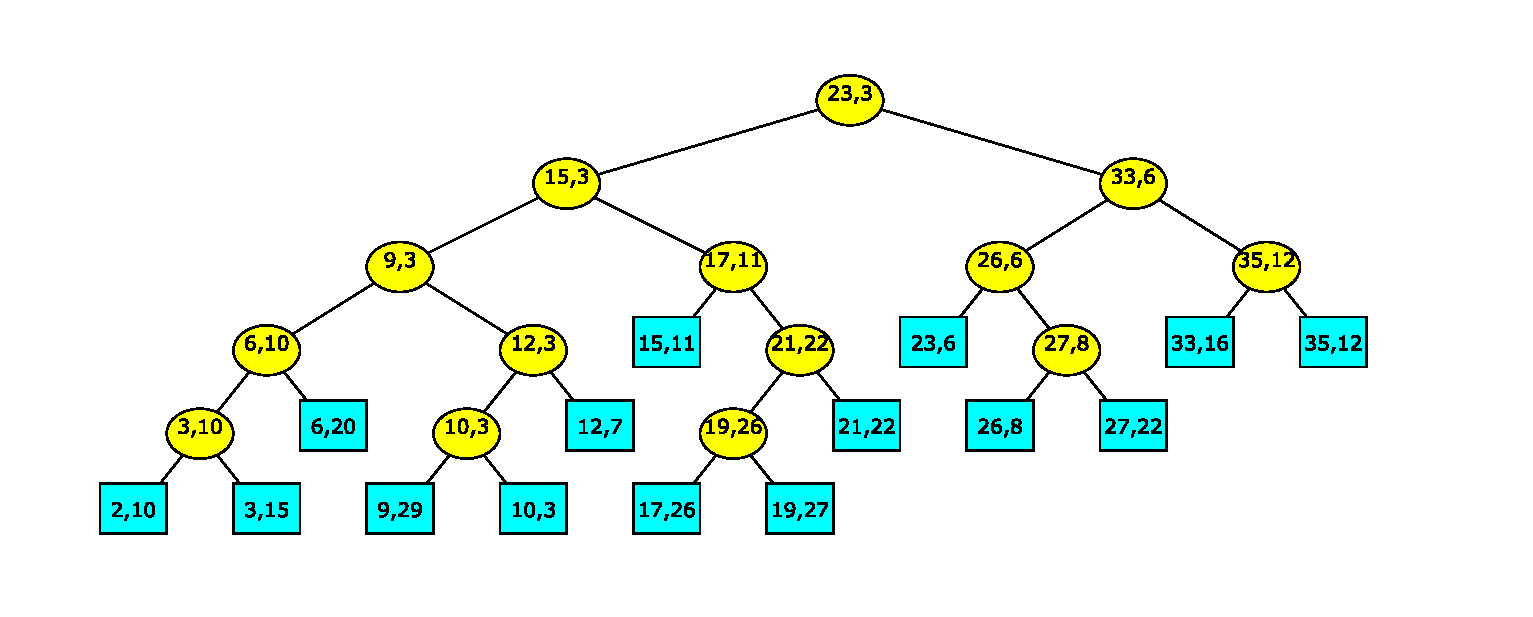
\includegraphics[scale=0.5]{pst}\\
  \caption{PST.}\label{fig:pst}
\end{figure*}

See Figure 1, in each node we only draw $q.x \& p.y$. So, as to
$v.q.x$, the structure is a 1-D range tree, whereas to the $v.p.y$,
the structure is a heap.
\section{Insertion}
\begin{theorem}
Insertion can be done in O($\log n$). 
\end{theorem}

See Algorithm 2 and
Figure 2.
\begin{figure*}[!h]
  \centering
  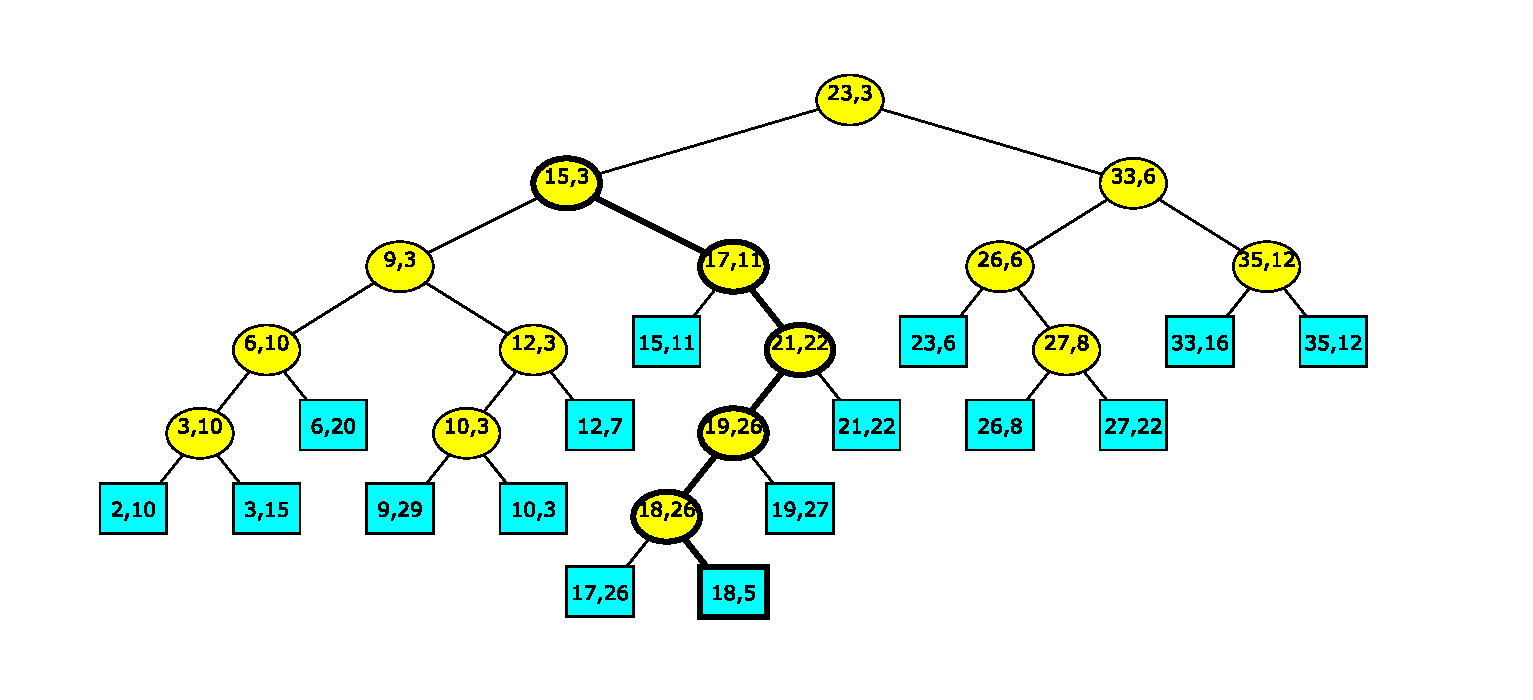
\includegraphics[scale=0.5]{pst_just_insert}\\
  \caption{Insertion before tournament.}\label{fig:pst_just_insert}
\end{figure*}

\begin{algorithm}[!h]
\caption{Insertion} \label{alg:pst_insert}
    \begin{algorithmic}[1]
     \REQUIRE a PST tree $T$ and a point $(x_1,y_1)$
     \STATE Find a leaf node to be inserted according to the $x_1$ value. say $v$.
     \STATE Create a new node $z$, and replace $v$ with $z$.
     \STATE Create a new node $w$ to be inserted.
     \STATE Make $v$ and $w$ be the children of $z$.
     \STATE Maintain the feature of Range Tree.
     Update $p$\ value of node $z$, and the first node whose right child is the node $z$'s father.
     \STATE Maintain the feature of Heap. Replay the tournament up with $w$ until it does not win.
     \COMMENT {Time Complexity of Steps above all is O($\log n$).}
     \STATE re-balancing the tree.
     \COMMENT {Time Complexity is O($\log n$). Detail discussions in the section Rotation.}
    \end{algorithmic}
\end{algorithm}

The insertion algorithm divided into two steps. Assume that the new
point is $(x_1,y_1)$. First step, we can determine the proper location
for the new point because we know that the priority search tree,
viewed in a one dimensional sense, maintains the property of a
binary search tree on the $q.x$ of the points. We traverse along a
single path from the root of the tree to a leaf node comparing the
$x_1$ to the $x$ coordinate of the point p represented by the given
internal node. If the $x_1$ is less than $x$ coordinate of the given
point $q$, we proceed to the left subtree otherwise we proceed to
the right subtree. When the first step of our insertion algorithm
reaches a leaf of the tree, we say this node $v$. we add a new
interior node $z$ in place of $v$, and make $v$ one of the children of
this new internal node $z$. Then we add a new leaf $w$ to the tree as
the other child, and store the new point $(v,w)$ in p, q value of
this leaf $w$.

For the second step of our insertion algorithm, we update the $p$, $q$
of the interior node to maintain the feature of Range Tree and Heap.
As to $q$ value on heap, there are two nodes to be updated, and one
is node $z$. The algorithm is below.
\begin{algorithm}[!h]
\caption{maintain the Range tree feature} \label{alg:rangetreefeature}
	\begin{algorithmic}[1]
	\STATE $z.q$ $\leftarrow$ $z.right.q$
	\STATE $tmp$ $\leftarrow$ $z.left$
	\WHILE{$tmp$ is not root and $tmp$ is its parent's left child}
	\STATE $tmp$ $\leftarrow$ $tmp.parent$
	\IF{$tmp$ is not root}
	\STATE $tmp.parent.q$ $\leftarrow$ $z.left.q$
	\ENDIF
	\ENDWHILE
	\end{algorithmic}
\end{algorithm}

As to p value, we implement a bottom-to-top tournament from node
$z$ until it does not win its sibling in tournament.

The reason why we keep a boolean value (win) is that we can use the
win/lose records to reduce the time of comparison, making the
tournament simple. In other words, if you have won A, you will win the
one which has been defeated by A, or vice versa.
\begin{figure*}[!h]
  \centering
  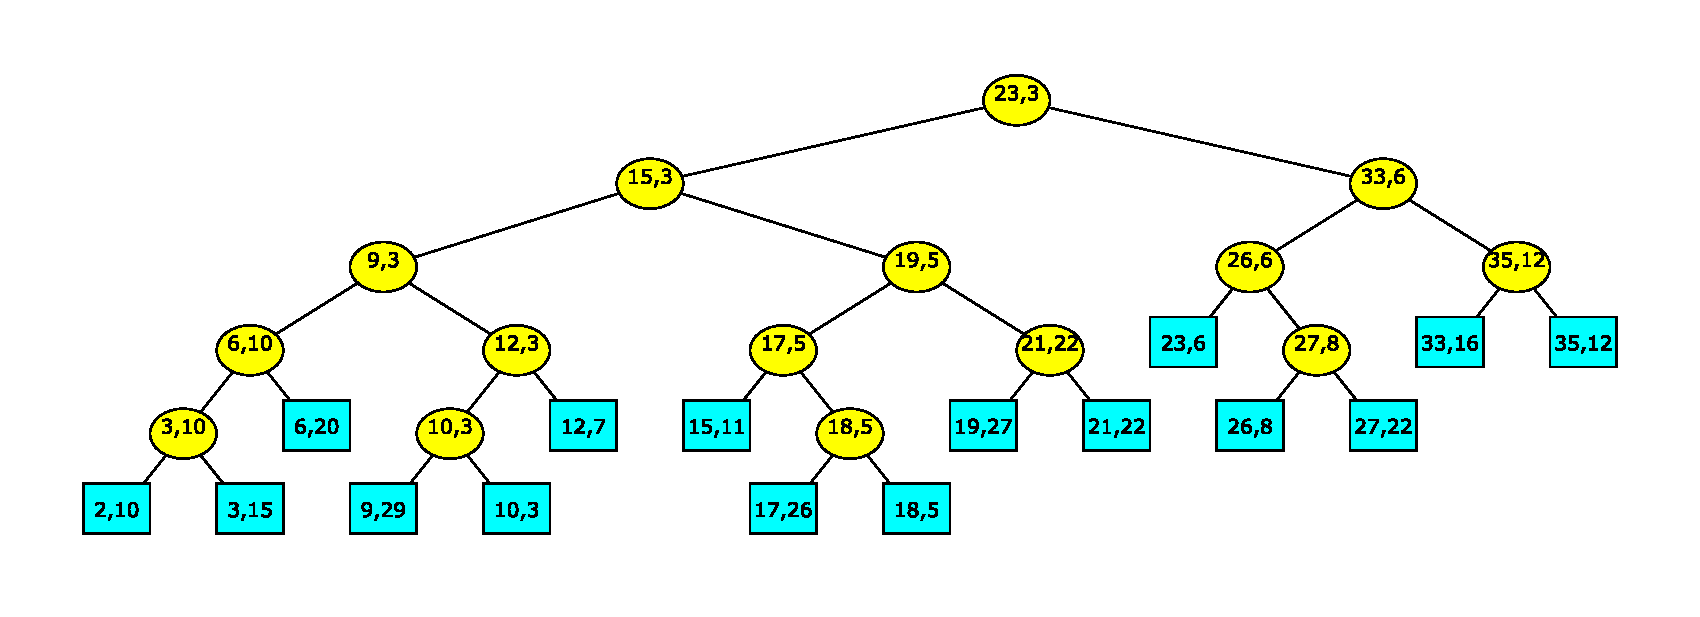
\includegraphics[scale=0.5]{pst_insert}\\
  \caption{Insertion after tournament and balancing}\label{fig:pst_insert}
\end{figure*}

So, the total time complexity is still O($\log n$).
\section{Deletion}

\begin{theorem}
Theorem: deletion can be done in O($\log n$).
\end{theorem}

The algorithm for deletion from the dynamic priority search tree is
straightforward and takes advantage of many of the techniques we
have already discussed. We must perform the following steps: (See
Algorithm 3.)
\begin{algorithm}[!h]
\caption{Deletion} \label{alg:pst_delete}
    \begin{algorithmic}[1]
    \REQUIRE a PST tree $T$ and a point $(x_1,y_1)$
    \STATE Find the leaf node to be deleted, say $v$. $z$ be the parent of $v$, and $w$ be the sibling of $v$.
    \STATE Replace $z$ with $w$. Delete $v$ and $z$.
    \STATE Maintain the feature of Range Tree.
    \STATE Maintain the feature of Range Tree.
    Replay the tournament up from $w$ until the defender is a winner.
    \COMMENT {Time Complexity of Steps above all is O($\log n$).}
    \STATE re-balancing the tree.
     \COMMENT {Time Complexity is O($\log n$). Detail discussions in the section Rotation.}
    \end{algorithmic}
\end{algorithm}
See figure 3. The total time complexity is still O($\log n$).

\section{Query}
There are two methods to deal with this range query
($[x_1:x_2],[-\infty:y]$) or ($[x:\infty],[-\infty:y]$) problem.
\subsection{Recursive method~\cite{CG_02} (we do not use, just an introduction)}
The main idea on recursive method is under below. We first search
for the node $v_{split}$ where the paths to $x_1$ and $x_2$
split.This node must be the common father of every solution. This is
done woth the following subroutine. Let $lc(v)$ and $rc(v)$ denote
the left and right child, respectively, of a node $v$.

\begin{algorithm}[!h]
\caption{FindSplitNode} \label{alg:find split node}
    \begin{algorithmic}[1]
    \REQUIRE a PST tree $T$ and two values $x_1,x_2$ with $x_1<x_2$
    \STATE $v$ $\leftarrow$ root($T$)
    \WHILE {v is not a left  and ($x_2<x_v$ or $x_1 \geq x_v$)}
        \IF{$x_2<x_v$}
        \STATE $v$ $\leftarrow$ $lc(v)$
        \ELSE
        \STATE $v$ $\leftarrow$ $rc(v)$
        \ENDIF
    \ENDWHILE
    \STATE RETURN $v$
    \end{algorithmic}
\end{algorithm}

Starting from $v_{split}$ we then follow the algorithm 5. Detail
discussion please see reference book~\cite{CG_02}.
\begin{algorithm}[!h]
\caption{RecursiveRangeQuery} \label{alg:recursive
method}
    \begin{algorithmic}[1]
    \STATE Starting from $v_{split}$
    \STATE Follow the search path of $lc(v)$. Report all the
leaves in the right subtree where path goes left.
    \STATE Follow the path of $(rc(v))$. Report the leaves in the left subtree of nodes where the path goes right.
    \STATE Check the points stored at the leaves where the paths end.
    \end{algorithmic}
\end{algorithm}


\subsection{Iterator method}
DPST iterator data strucure is under below. This iterator is different 
with other iterator for it stores not only a pointer, but also a value.\\
\begin{verbatim}
iterator{
    Node * node;
    int y;
}
\end{verbatim}
LowerBound() returns an node iterator which
is the leftmost leaf node of the whole solutions and iterator++
moves to next solution, while UpperBound() returns an node
iterator which is the rightmost leaf node of the solutions and
iterator-- moves to previous solution. It obviously require less
storage spaces than that in recursive method. So, we could traverse
the solutions like this way below in our program.
\begin{algorithm}[!h]
\caption{TraverseTheSolutions} \label{alg:traversing}
	\begin{algorithmic}[1]
	\STATE $it1$ $\leftarrow$ LowerBound($v$,$x_1$,$x_2$,$y$)
	\STATE $it2$ $\leftarrow$ UpperBound($v$,$x_1$,$x_2$,$y$)
	\REPEAT
	\STATE some processed we want to do
	\STATE $it1++$
	\UNTIL{$it1==it2$} 
	\end{algorithmic}
\end{algorithm}
Firstly, we find the $v_{split}$ node just like we discussed in
previous subsection. We take the LowerBound(int x1,int x2,int y)
function in detail, and LowerBound(int x1,int x2,int y)
UpperBound(int x, int y) UpperBound(int x,int y) could be easily
derived from this idea.
\begin{algorithm}[!h]
\caption{LowerBound} \label{alg:find lowerbound}
    \begin{algorithmic}[1]
    \REQUIRE a PST tree $T$ and three values $x_1,x_2$ with
$x_1<x_2$, and $y$
    \STATE $v$ $\leftarrow$ FindSplitNode($T$)
    \RETURN iterator(LowerBoundRecur($v$,$x_1$,$x_2$,$y$), $y$)
    \end{algorithmic}
\end{algorithm}

\begin{algorithm}[!h]
\caption{LowerBoundRecur} \label{alg:find lowerboundrecur}
    \begin{algorithmic}[1]
    \REQUIRE a PST node $v$ and three values $x_1,x_2$ with
$x_1<x_2$, and $y$
    \STATE $tmp$ $\leftarrow$ NULL
    \WHILE {$v$ is not NULL}
	\IF{$y<v.p.y$}
        \RETURN tmp //not found
        \ENDIF
        \IF{v is leaf}
            \IF{!$(v.q.x<x_1)$ and !$(v.q.x>x_2)$}
                \RETURN x //found
	    \ELSE
                \RETURN tmp //not found
            \ENDIF
	\ENDIF
	\IF{!$(v.q.x<x_1$)}
	\STATE $tmp$ $\leftarrow$ LowerBoundRecur($v$,$x_1$,$x_2$,$y$);
	\ENDIF
	\IF{tmp is not NULL}
            \RETURN tmp //found
        \ENDIF
	\STATE $v$ $\leftarrow$ $rc(v)$
	\ENDWHILE
     \RETURN tmp
\end{algorithmic}
\end{algorithm}

Then, we list the iterator algorithm below.

\begin{algorithm}[!h]
\caption{operator$++$} \label{alg:operator++}
	\begin{algorithmic}[1]
	\REQUIRE a PST node iterator $it$
	\REPEAT
	\STATE increment($it$)
	\IF{$it.node$ is NULL}
	\STATE Break
	\ENDIF
	\UNTIL($it.node$ is a leaf and $it.node.y <= y$)
	\end{algorithmic}
\end{algorithm}

\begin{algorithm}[!h]
\caption{increment($iterator$)} \label{alg:increment}
	\begin{algorithmic}[1]
	\REQUIRE a PST node iterator $it$
	\IF{$it.node$ is leaf}
		\WHILE{$it.node$ is its parent's right node and $it.node$ is not root}
		\STATE	$it.node$ $\leftarrow$ $parent(it.node)$
		\ENDWHILE
		\STATE	$it.node$ $\leftarrow$ $parent(it.node)$
	\ELSE
		\STATE	$it.node$ $\leftarrow$ $rc(it.node)$
		\WHILE{$it.node.y >= it.y$ and $it.node$ is not leaf}
		\STATE	$it.node$ $\leftarrow$ $lc(it.node)$
		\ENDWHILE
	\ENDIF
	\end{algorithmic}
\end{algorithm}

\section{Re-balancing}
\subsection{Rotation}
\begin{theorem}
At most one replay is necessary for each single tree rotation.
\end{theorem}
\begin{proof} 
Consider left rotation. Let x, y be the nodes to
be rotated where y is the right child of x. ly and ry are the left
child and right child of y respectively. lx is the left child of x.

Case 1: y is not a winner

It implies lx must be a winner and hence ly and ry must both be
losers after rotation. No replay is necessary.

\begin{figure}[!h]
  \centering
  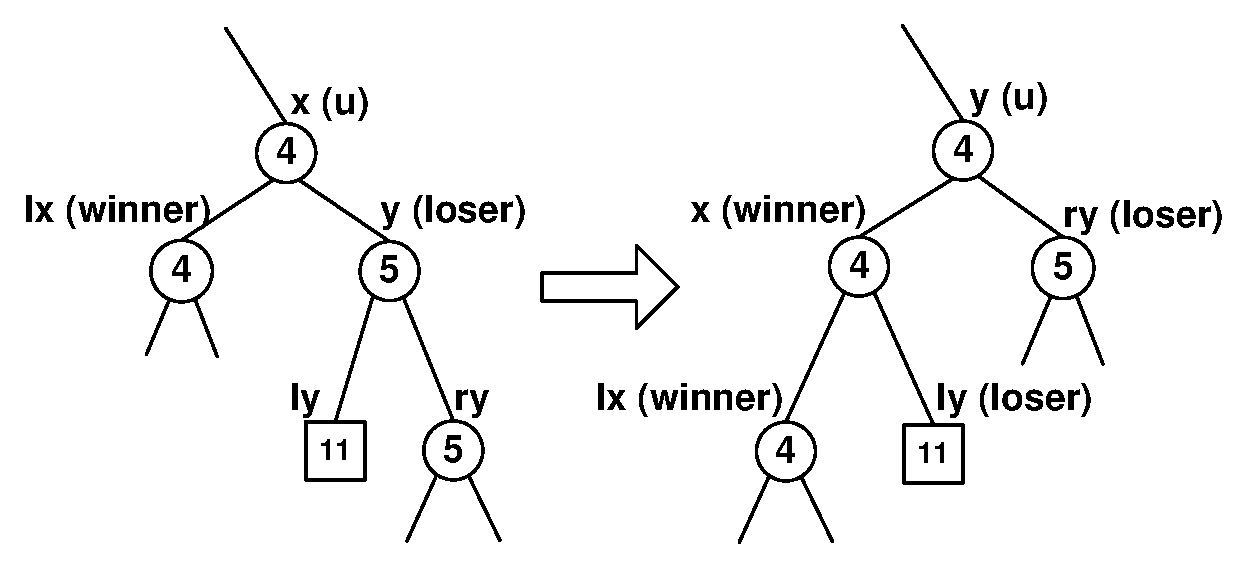
\includegraphics[scale=0.4]{case_1}\\
  \caption{Case 1.}\label{fig:case_1}
\end{figure}

Case 2: y is a winner

Case 2.1: ly is a winner It implies x will also be a winner.
Statuses of other nodes are unchanged after rotation. No replay is
necessary.
\begin{figure}[!h]
  \centering
  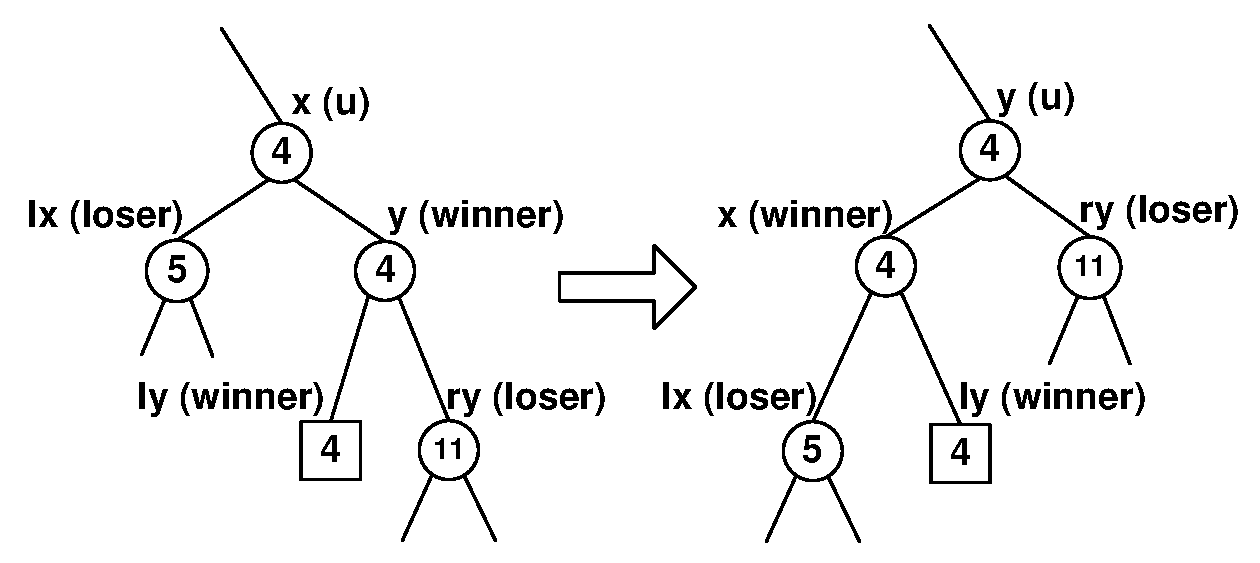
\includegraphics[scale=0.4]{case_2_1}\\
  \caption{Case 2.1.}\label{fig:case_2_1}
\end{figure}

Case 2.2: ly is not a winner It implies both lx and ly are $>$= 4,
ry will be a winner. lx and ly need to be replayed
\begin{figure}[!h]
  \centering
  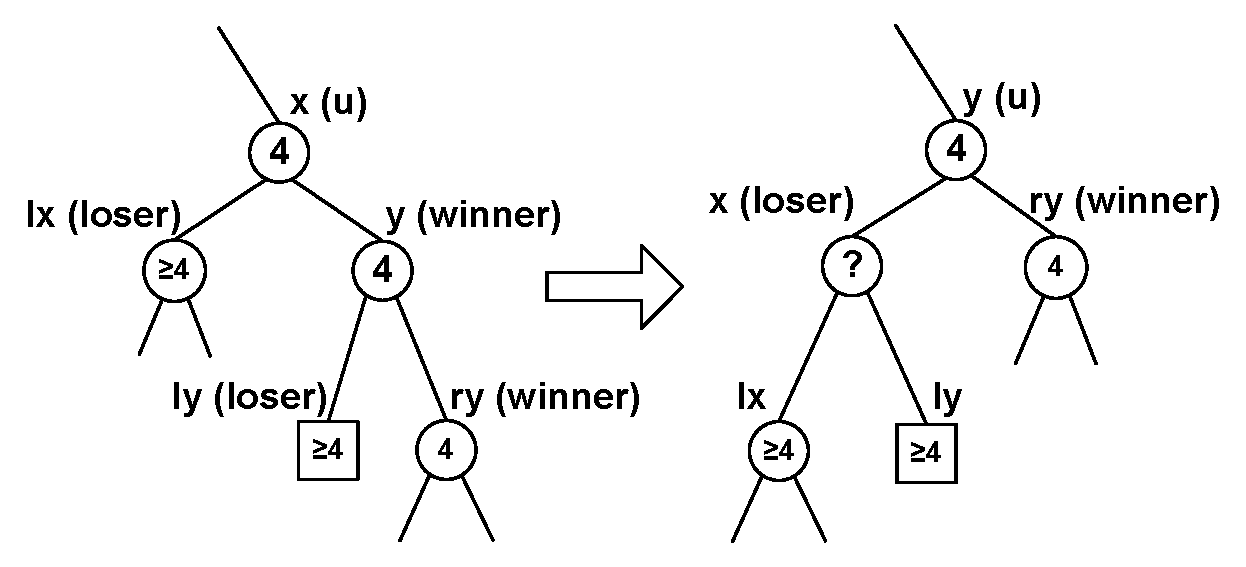
\includegraphics[scale=0.4]{case_2_2}\\
  \caption{Case 2.2.}\label{fig:case_2_2}
\end{figure}
\end{proof}

The time complexity is O(1).
\subsection{Insertion \& Deletion time complexity}
In conclusion, one time rotation takes O(1) while original
version~\cite{Edward_04} may take O($\log n$) in worse case, for it
will update some values from current node to bottom. If insertion or
deletion needs rotate O($\log n$) times, then the total time is
$1+2+3+...+\log n = \log n(\log n+1)/2$. Time complexity is
O$(\log^2 n)$ in such worst case. Our version is O($\log n$)!

\section{Experimental Results}
In this section, we will do some experiments to support our claims
above all. The experimental environment is a linux server, with 2.80GHz Intel(R)
Xeon(TM) CPU, and 8GB memory. We have just implemented two versions dynamic PST,
besides our version, the one is proposed by ~\cite{Edward_04}, and we
also implement a Radix PST (RPST)~\cite{Edward_04}, which is a PST without
re-balancing. We compared these three versions with running time 
in insertion, deletion, and query.

\subsection{Insertion}
We compared the running time that inserting ten nodes
in a certain number, and the total time that creating the whole tree
by one by one insertion with certain node number.\\
We choose the random point distributed uniformly in the plane.\\

\begin{table}[ht]
\begin{tabular}{|p{1.1cm}|p{0.8cm}|p{0.8cm}|p{0.8cm}|p{0.8cm}|p{0.8cm}|p{0.8cm}|}
\hline node & \multicolumn{3}{|c|}{inserting ten nodes ($\mu$s)} & \multicolumn{3}{|c|}{total running time (ms)}\\
\cline{2-7}
number & our DPST & ori DPST  & RPST & our DPST & ori DPST & RPST\\
\hline 1000 & 5 & 6 & 9 & 0.5 & 0.66 & 0.3\\
\hline 5000 & 14 & 16 & 5 & 3.0 & 4.1 & 1.7\\
\hline 10000 & 8 & 9 & 5 & 6.6 & 8.8 & 3.7\\
\hline 50000 & 14 & 28 & 7 & 62 & 116 & 25\\
\hline 100000 & 17 & 22 & 10 & 143 & 183 & 66\\
\hline 500000 & 26 & 60 & 17 & 1186 & 1342 & 572\\
\hline
\end{tabular}
\end{table}

Then we choose the random point distributed nonuniformly in the plane, such as restricting the point into a narrow slot.\\


\begin{table}[ht]
\begin{tabular}{|p{1.1cm}|p{0.8cm}|p{0.8cm}|p{0.8cm}|p{0.8cm}|p{0.8cm}|p{0.8cm}|}
\hline node & \multicolumn{3}{|c|}{inserting ten nodes (us)} & \multicolumn{3}{|c|}{total running time (ms)}\\
\cline{2-7}
number & our DPST & ori DPST  & RPST & our DPST & ori DPST & RPST\\
\hline 1000 & 5 & 6 & 11 & 0.49 & 0.67 & 0.56\\
\hline 5000 & 11 & 8 & 5 & 2.9 & 4.0 & 2.2\\
\hline 10000 & 7 & 11 & 5 & 6.6 & 8.8 & 5.2\\
\hline 50000 & 13 & 23 & 28 & 57 & 75 & 60.8\\
\hline 100000 & 16 & 19 & 61 & 137 & 180 & 294\\
\hline 500000 & 28 & 29 & 369 & 1082 & 1377 & 9146\\
\hline
\end{tabular}
\end{table}

The insertion running time of our version is less than that of original version no matter the random point selecting. However, as to the RPST, due to its unbalancing and the random choosing of the point, the performance of RPST varies largely.However, actually, the unbalanced RPST is not a wise choice in application.

\subsection{Deletion}
We compared the running time that deleting ten nodes in
a certain number, and the total time that deleting the whole tree
one bye one with certain node number.\\
We choose the random point distributed uniformly in the plane.\\

\begin{table}[ht]
\begin{tabular}{|p{1.1cm}|p{0.8cm}|p{0.8cm}|p{0.8cm}|p{0.8cm}|p{0.8cm}|p{0.8cm}|}
\hline node & \multicolumn{3}{|c|}{inserting ten nodes (us)} & \multicolumn{3}{|c|}{total running time(ms)}\\
\cline{2-7}
number & our DPST & ori DPST  & RPST & our DPST & ori DPST & RPST\\
\hline 1000 & 7 & 9 & 5 & 0.29 & 0.4 & 0.2\\
\hline 5000 & 9 & 11 & 8 & 1.90 & 2.5 & 1.3\\
\hline 10000 & 13 & 18 & 6 & 6.56 & 6.7 & 2.9\\
\hline 50000 & 21 & 40 & 13 & 56.2 & 87.0 & 24.1\\
\hline 100000 & 26 & 28 & 18 & 143 & 176& 70\\
\hline 500000 & 34 & 58 & 21 & 1090 & 1380 & 614\\
\hline
\end{tabular}
\end{table}

Then we choose the random point distributed nonuniformly in the plane.\\

\begin{table}[ht]
\begin{tabular}{|p{1.1cm}|p{0.8cm}|p{0.8cm}|p{0.8cm}|p{0.8cm}|p{0.8cm}|p{0.8cm}|}
\hline node & \multicolumn{3}{|c|}{inserting ten nodes (us)} & \multicolumn{3}{|c|}{total running time (ms)}\\
\cline{2-7}
number & our DPST & ori DPST  & RPST & our DPST & ori DPST & RPST\\
\hline 1000 & 7 & 9 & 5 & 0.29 & 0.40 & 0.30\\
\hline 5000 & 10 & 13 & 8 & 1.90 & 2.70 & 1.70\\
\hline 10000 & 16 & 19 & 11 & 4.87 & 7.20 & 3.84\\
\hline 50000 & 23 & 29 & 36 & 62.4 & 76.0 & 63.4\\
\hline 100000 & 27 & 31 & 74 & 145 & 189 & 317\\
\hline 500000 & 37 & 44 & 349 & 1081 & 1224 & 9017\\
\hline
\end{tabular}
\end{table}

The conclusion is similar to insertion's.
\subsection{Query}
In this table, we compared the running time traversing the whole
solutions with certain node number.

\begin{table}[ht]
\begin{tabular}{|p{1.2cm}|p{1.1cm}|p{1.1cm}|p{1.1cm}|p{1.1cm}|}
\hline node number & solution number & \multicolumn{3}{|c|}{running time (us)}\\
\cline{3-5}
    && our DPST & ori DPST & RPST\\
\hline 10000 & 1 & 3 & 6 & 5\\
\cline{2-5}      & 2 & 4 & 7  & 4\\
\cline{2-5}      & 7 & 6 & 8 & 11\\
\cline{2-5}      & 17 & 8 & 13 & 16\\
\hline 100000 & 12 & 11 & 14 & 11\\
\cline{2-5}      & 23 & 25 & 19  & 17\\
\cline{2-5}      & 127 & 58 & 52 & 39\\
\cline{2-5}      & 275 & 117 & 101 & 86\\
\hline 1000000 & 27 & 20 & 25 & 20\\
\cline{2-5}      & 125 & 75 & 65  & 46\\
\cline{2-5}      & 256 & 187 & 100 & 78\\
\cline{2-5}      & 520 & 277 & 198 & 169\\
\hline
\end{tabular}
\end{table}

When the solution number is small, our version takes less time than
original version, otherwise, original one is better. However, fortunately, we always meet the former situations.

\subsection{A complete example}
Let us now consider a complete example of insertion, deletion and
query. We implement a line sweeping algorithm to find out all the
overlapped rectilinear rectangles in plane. The main idea of the algorithm is mapping the intevals of axis to the points of a plane, see [].\\
We create the random rectangles about $20*60000$, 60000 means that about 60000 rectangles are intersected by the sweeping line.\\


\begin{table}[ht]
\begin{tabular}{|p{1.2cm}|p{1.2cm}|p{1.1cm}|p{1.1cm}|p{1.1cm}|}
\hline rectangle number & overlaped number & \multicolumn{3}{|c|}{running time (s)}\\
\cline{3-5}
    && our DPST & ori DPST & RPST\\
\hline 1380267 & 44090  & 3.98 & 4.93 & 2.34\\
\cline{2-5}      & 194935 & 4.89 & 6.17  & 2.78\\
\cline{2-5}      & 637177 & 6.17 & 6.31  & 2.90\\
\cline{2-5}      & 2444898 & 8.68 & 7.00  & 3.33\\
\cline{2-5}      & 12871654 & 13.1 & 9.60  & 5.07\\
\cline{2-5}      & 44530339 & 22.7 & 15.7  & 8.63\\
\hline
\end{tabular}
\end{table}

We create the random rectangles about $10*10000$, 10000 means that about 10000 rectangles are intersected by the sweeping line. The reason why we do this is that changing the uniformity of the mapping points, then we will notice the varying performance of RPST.\\



\begin{table}[ht]
\begin{tabular}{|p{1.2cm}|p{1.2cm}|p{1.1cm}|p{1.1cm}|p{1.1cm}|}
\hline rectangle number & overlaped number & \multicolumn{3}{|c|}{running time (s)}\\
\cline{3-5}
    && our DPST & ori DPST & RPST\\
\hline 98371 & 1583  & 0.078 & 0.122 & 0.092\\
\cline{2-5}      & 2464 & 0.082 & 0.127  & 0.097\\
\cline{2-5}      & 10669 & 0.110 & 0.144  & 0.105\\
\cline{2-5}      & 34111 & 0.134 & 0.161  & 0.120\\
\cline{2-5}      & 127567 & 0.218 & 0.252  & 0.287\\
\hline
\end{tabular}
\end{table}

In this example, if overlapped rectilinear rectangles number is small, our version is better than original version. However, as the increasing of overlapped rectangles, the original version takes advantage. As to the RPST, it seems that RPST is much better than other two. 
But its performance depends on the uniformity of the points, it may be degenerated to a list in the actual application, if so, the time complexity will be very worse. Just like we prefer red-black binary tree than normal binary tree. Readers should know the pros and cons between balanced and unbalanced one.

\section{Applications}
In[], a list of applications are described. The main applications
are for interval set. With plane sweeping, dynamic PST can used for
finding all overlapping of a set if axis-parallel rectangles, Figure 7. For
example, in global placement. In~\cite{DAC_05},VLSI layout
compaction use RPST. It can be used for constructing conflict
graphics in many applications such as phase-shift
masking (PSM)~\cite{PSM_05}.

\begin{figure}[!h]
  \centering
  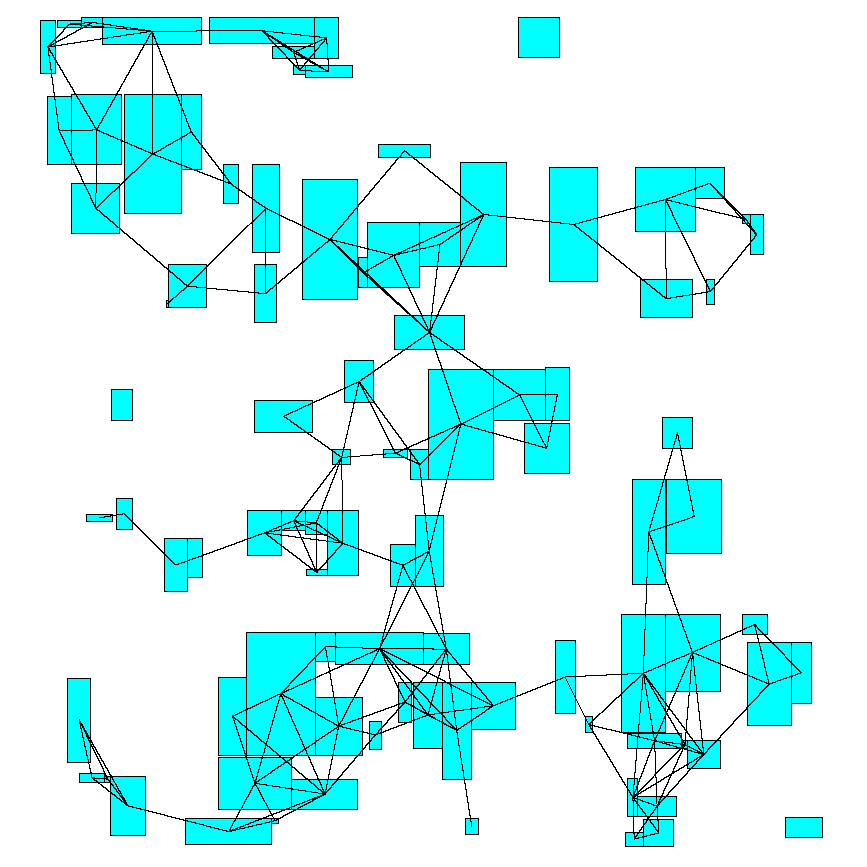
\includegraphics[scale=0.5]{conflict}\\
  \caption{PST.}\label{fig:conflict}
\end{figure}

\section{Conclusion}
In this paper we proposed an data structure, the Dynamic Priority
Search Tree, and its original version. It is particularly for 2-D
range query in form of ($[x1:x2],[-\infty:y]$). Its dynamic
insertion and deletion, and the ability to remain balanced make it a
more suitable data structure compared to other structures developed
for the same purpose, such as Radix Priority Search Tree. We have
shown, through the performance analysis, that the dynamic PST is
efficient for all the major operations it performs. The original one
takes O($\log^2n$) for insertion and deletion in worst case, while
the improved one takes O($\log n$) for insertion and deletion in
worst case. They both take O($k+\log n$) for search, occupy O($n$)
space usage. And the other important feature is that our version
made easy.

\bibliographystyle{unsrt}
\bibliography{ref-PST}

\end{document}
